
\newrefcontext[sorting=ynt]

\lettrine{A}{nimal} societies --- individual associations in a spatio-temporal context --- emerge from complex interactions between local ecological conditions and individual behavioural strategies \citep[][]{whitehead2008,tanner2012,webber2018}.
While such associations can yield useful social information about resource availability \citep{danchin2004,dall2005,gil2018}, they also provide opportunities for the transmission of infectious pathogens \citep[][]{krause2002,weinstein2018,romano2020,albery2021,cantor2021,romano2021}.
Individuals must therefore balance the costs and benefits of socialising when deciding how to move.
Movement strategies that incorporate social information --- the presence and status of neighbours --- can facilitate or reduce spatial associations, or encounters \citep{danchin2004,dall2005,nathan2008a,gil2018,webber2018,webber2022}.
Movement is therefore an important mechanism linking landscape spatial structure and individual distributions with the emergent structure of animal societies.
Together, they influence the dynamics of disease outbreaks in animal populations \citep{white2018a,romano2020,romano2021}, and outbreaks may in turn cause cascading effects on landscape and community ecology \citep{monk2022}.

The introduction of pathogens to animal societies often leads to rapid reductions in associations among individuals \citep[][]{romano2020}, due to a combination of mortality-induced decreases in population density \citep[e.g.][]{fereidouni2019} and adaptive behavioural responses that reduce encounter rates \citep{stroeymeyt2018,romano2020,stockmaier2021}.
Importantly, when a novel pathogen is first introduced into a population, such as during a spillover event, individuals may have no prior experience of cues that indicate infection \citep{power2004}, making fine-tuned adaptive individual or social avoidance responses less likely.
If they reduce fitness, novel pathogens spreading through host-host contacts may select against host social behaviour, ultimately selecting against social connectivity itself \citep{altizer2003,cantor2021,romano2021,poulin2021,ashby2022}.
This selective pressure may be modulated by landscape productivity \citep{hutchings2006} and the benefits of grouping \citep[][]{almberg2015,ezenwa2016}, especially if these can boost fitness in a way that offsets the cost of infection.
Multiple animal taxa currently face novel pathogen outbreaks \citep{blehert2009,globconsorth5n82016,fereidouni2019,scheele2019}, and this number is likely to grow in the near future due to climate change \citep{sanderson2020,carlson2021}.
It is therefore especially important to know how rapid evolutionary changes following pathogen introduction will be, as well as their effect on social systems and the transmission of animal culture \citep{cantor2021, cantor2021a}.

Analytical models suggest that animal sociality evolves to balance the value of social information against the risk of pathogen transmission \citep[][]{bonds2005,prado2009,ashby2022}.
However, these models make a number of simplifying assumptions, including homogeneous populations, and single parameters for sociality \citep[][]{bonds2005,prado2009,ashby2022}.
In reality, sociality is an emergent outcome of spatially heterogenous environmental conditions and often substantial within-population heterogeneity in behaviour \citep{tanner2012, wolf2012}.
Epidemiological models based on contact networks allow for heterogeneity in pairwise associations; however, these models are sensitive to the network formation process, and sampling biases in empirical data collection can complicate their parameterisation \citep[][]{white2017}.
Similar to analytical models, network models make assumptions about individuals' positions in a social network, when these positions are actually emergent outcomes of social movement -- how and where to move in relation to other individuals.
Simple models also gloss over the mechanisms underlying sociality, and especially ignore the role of animal movement strategies and the spatial context of animal associations and pathogen transmission \citep{albery2021}.
Mechanistic, individual-based simulation models can incorporate substantial ecological detail, including an explicit spatial setting \citep{deangelis2019}, individual variation in movement strategies \citep{spiegel2017,lunn2021}, and realistic disease transmission \citep{white2018, scherer2020, lunn2021}.
Yet mechanistic movement-disease models thus far focus on immediate ecological outcomes, such as infection persistence, and do not have an evolutionary component \citep{white2018,scherer2020,lunn2021}.
Limiting movement-disease models to an ecological scale could miss important feedbacks between the ecological outcomes of infectious disease and the consequences for the evolution of host behaviour \citep{cantor2021}.
Incorporating an evolutionary component to movement-disease models could allow predictions on the long-term consequences of wildlife disease outbreaks, such as changes in the the emergent structure of animal societies.

We examined the eco-evolutionary consequences of the introduction of a pathogen into a novel host population, such as during cross-species spillover, a scenario of increasing frequency and global concern \citep{blehert2009,globconsorth5n82016,fereidouni2019,scheele2019,sanderson2020,carlson2021,kuchipudi2022}.
We developed a mechanistic, evolutionary, spatially-explicit, individual-based simulation model in which we introduced an infectious pathogen to populations that had already evolved movement strategies in a foraging context \citep[see model code, analysis code, and reference data:][]{gupte2022,gupte2022a,gupte2022b}.
In our model, the depletion of patchily distributed, discrete food items makes the use of social information key to finding food (see \textit{Supplementary Material Fig. 1 -- 2}; see also \citealt{gupte2021a}).
%%
We investigated three questions: \textit{(i)} How does the introduction of a novel pathogen affect the evolution of animals' social movement strategies?
\textit{(ii)} How do pathogen-adapted movement strategies affect the emergent structure of animal societies?
\textit{(iii)} How are evolutionary responses to pathogen introduction shaped by ecological factors, such as landscape productivity and the cost of infection?
%%
We compared how social information was used in movement strategies evolved before and after pathogen introduction, and the ecological outcomes for individual intake, movement, and associations with other foragers.
We constructed proximity based social networks from individuals' movements \citep{whitehead2008,white2017,wilber2022}.
We used network epidemiological models to examine whether pathogen-adapted populations were more resilient to the spread of infectious disease than their pathogen-naive ancestors \citep[][]{white2017,stroeymeyt2018,wilber2022}.
We examined the effect of two important model parameters, landscape productivity ($R$) and infection cost ($\delta E$), by running our model over nine different combinations of $R$ and $\delta E$.
Overall, we provide a theoretical framework and reference implementation for the study and prediction of the evolutionary consequences of pathogen introduction for animal populations in a spatial context.

\section*{Model and Analysis}

We implemented an individual-based simulation model to represent foraging animals (`foragers') seeking discrete, immobile, depleteable food items \citep[as in][see \textit{Supplementary Material Fig. 1 -- 2}]{spiegel2017,gupte2021a}.
Food items are distributed over a two-dimensional, continuous-space resource landscape with wrapped boundaries (a torus).
Our model, similar to previous eco-evolutionary individual based models \citep{getz2015, netz2021a, gupte2021a}, has two distinct timescales: (1) an ecological timescale comprising of \textit{T} timesteps that make up one generation ($T$ = 100 by default), and (2) an evolutionary timescale consisting of 5,000 generations ($G$).
At the ecological timescale, individuals sense local counts of food items and competitors, move according to inherited movement strategies, and forage for food.
At the same timescale, individuals that carry an infectious, fitness-reducing pathogen, may, when in close proximity with uninfected individuals, pass on the pathogen with a small probability (see \textit{Pathogen Transmission and Disease Cost}).
At the evolutionary timescale, individuals reproduce and transmit their movement strategies (see \textit{Starting Location and Inheritance of Movement Rules}) to the their offspring. The number of offspring is linked both to individuals' success in finding and consuming food items, and to the duration that they were infected by the pathogen at the ecological timescale.
The model was implemented in R and C++ using Rcpp \citep{rcoreteam2020,eddelbuettel2013}, using R-trees from the \textit{Boost.Geometry} C++ library for spatial computations (\textit{www.boost.org}), and can be found at \textit{github.com/pratikunterwegs/pathomove}.

\subsection*{Distribution of Food Items}

Our landscape of 60 $\times$ 60 units contains 1,800 discrete food items, which are clustered around 60 resource `kernels', for a resource density of 0.5 items per unit\textsuperscript{2} (see \textit{Supplementary Material Fig. 1 -- 2}).
This prevents synchronicity in the availability and regeneration of food items.
Each available food item can be sensed and harvested by foraging individuals (see below).
Once harvested, another food item is regenerated at the same location after a fixed regeneration time $R$, which is set at 50 timesteps by default; alternative values of 20 and 100 timesteps represent high and low productivity landscapes respectively.
Food item regeneration is delinked from population generations.
Thus the actual number of available food items is almost always in flux.
In our figures and hereafter, we chose to represent $R$ as the number of times a food item would regenerate within the timesteps in a single generation $T$ (default = 100), resulting in $R$ values of 1, 2, and 5 for regeneration times of 100, 50 (the default), and 20 timesteps.
Items that are not harvested remain on the landscape until they are picked up by a forager.
Each food item must be processed, or `handled', by a forager for $T_H$ timesteps (the handling time, default = 5 timesteps) before it can be consumed \citep{ruxton1992,gupte2021a}.
The handling time dynamic is well known from natural systems in which there is a lag between finding and consuming a food item \citep{ruxton1992}, and may be caused by the need to extract edible portions from inedible structures, such as mussels from their shells, or seeds from their casings.

\subsection*{Individual Foraging and Movement}

\paragraph*{Foraging} Individuals forage in a randomised order, harvesting the first available food item within their movement and sensory range ($d_S$ = $d_M$, a circle with a radius of 1 unit (see \textit{Supplementary Material Fig. 1 -- 2}).
A forager at the edge of the landscape senses food items (and other foragers, see below) on the wrapped landscape.
Once harvested, the item is no longer available to other individuals, leading to exploitation competition among nearby foragers.
Furthermore, the location of the item also yields no more cues to other foragers that an item will reappear there, reducing direct cues by which foragers can navigate to profitable clusters of food items.
Individuals that harvest a food item must handle it for $T_H$ timesteps (default = 5 timesteps), while 
All individuals not handling a food item are considered idle \citep{ruxton1992,gupte2021a}.
As handlers are immobilised at the location where they encountered food, they may be good indirect indicators of the location of a resource cluster \cite[`social information'][]{danchin2004,romano2020,gupte2021a}.
Once individuals finish handling a food item, they return to the non-handling, searching state.

\paragraph*{Movement} Our model individuals move in small, discrete steps of fixed size ($d_M$ = 1 unit).
Each step is chosen based on the individuals' assessment of local environmental cues, and this assessment is made using evolved movement strategies \citep[as in][]{netz2021a,gupte2021a}.
First, individuals scan their current location, and five equally spaced points located on the arc of a circle with a radius of 0.5 units ($\sim$1\% of the landscape's side).
around their position, at a distance of 1 unit for three cues ($d_S$, see \textit{Supplementary Material Fig. 1 -- 2}): the number of food items ($F$), the number of foragers handling a food item (`handlers': $H$) and the number of idle foragers not handling a food item (`non-handlers': $N$).
Individuals assign a suitability \citep[see][]{netz2021a,gupte2021a} to their current position and each of the five locations, using their inherited preferences for each of the cues: $S = s_FF + s_HH + s_NN$ + $\epsilon$.
The preferences $s_F$, $s_F$, and $s_N$ for each of the three cues are heritable from parents to offspring, while $\epsilon$ is a very small error term drawn for each location, to break ties among locations.
The values of each of the cue preferences \emph{relative to each other} determine individuals' movement strategies \citep{gupte2021a}
All individuals move simultaneously to the location to which they have assigned the highest suitability (akin to step-selection; \citealp{avgar2016}); this may be their current location, in which case individuals are stationary for that timestep.
Since individuals may differ in their inherited preferences for each of the three cues, two individuals at the same location may make quite different movement decisions based on the same local cues.
Handlers, however, are considered immobile and do not make any movement decisions.

\subsection*{Pathogen Transmission and Disease Cost}

We modelled circumstances that are expected to become increasingly common due to rapid global changes; the population evolves for $3/5$\textsuperscript{th} of the simulation (until $G$ = 3,000; of 5,000) in the absence of a pathogen, after which, a pathogen is introduced in each generation until the end of the simulation ($G$ = 5,000).
We modelled an infectious pathogen with highly simplified dynamics, which can be transmitted from an infected to a susceptible individual with a low probability $p$ (default $p$ = 0.05).
This transmission is only possible when the two individuals are within a the transmission distance, $d_\beta$.
For simplicity, we set $d_\beta$ to be the movement range (1 unit).
Once transmitted, the pathogen is assumed to cause a chronic disease which reduces host energy stores by a fixed amount called $\delta E$ in every following timestep; $\delta E$ is set to 0.25 by default (alternative values: 0.1, 0.5).
Since such infectious contact events can periodically re-occur in natural environments, we set up our model such that the pathogen was introduced to 4\% of individuals (N = 20) in each generation.
This is necessary to kick-start the pathogen-movement eco-evolutionary feedback dynamics.
This is also realistic, as populations may repeatedly acquire pathogens through external sources, such as infected individuals of other, spatially overlapping species \citep[e.g.][]{kuchipudi2022}.

\subsection*{Starting Location and Inheritance of Movement Rules}

For simplicity, we considered a population of haploid individuals with discrete, non-overlapping generations, and asexual inheritance.
At the end of the parental generation, the net lifetime energy of each individual was determined as the difference of the total energy gained through food intake and the energy lost through infection. 
In \textit{Supplementary Material Section 3.2}, we also consider an alternative implementation in which the pathogen reduces the value of each food item by a certain percentage.
The parental population produced an offspring population (of the same size) as follows: to each offspring, a parent was assigned at random by a weighted lottery, with weights proportional to lifetime net energy \citep{netz2021a, gupte2021a}.
This way, the expected number of offspring produced by a parent is proportional to the parent's lifetime net energy.
The movement decision-making cue preferences $s_F$, $s_H$, and $s_N$ are subject to independent random mutations with a probability of 0.001.
The mutational step size (either positive or negative) is drawn from a Cauchy distribution with a scale of 0.01 centred on zero.
Thus, there can be a small number of very large mutations, while the majority of mutations are small.
As in real ecological systems, individuals in the new generation are intialised around the location of their parent (within a standard deviation of 2.0), and thus successful parents give rise to local clusters of offspring (see an alternative implementation in \textit{Supplementary Material Section 3.1}).

\subsection*{Model Output}

\paragraph{Social Information Use}

To understand the evolution of movement strategies, and especially how individuals weighed social information, we exported the population's evolved cue preferences in every second generation.
We classified individuals based on how they used social information --- the presence and status of competing foragers --- into four social movement classes: (1) agent avoiding, if $s_H, s_N < 0$, (2) agent tracking, if both $s_H, s_N > 0$, (3) handler tracking, if $s_H > 0, s_N < 0$, and (4) non-handler tracking, if $s_H < 0, s_N > 0$.
We calculated the relative importance of social cues --- $H, N$ --- to each individual's movement strategy as $ SI_{imp} = (|s_H| + |s_N|) / (|s_H| + |s_N| + |s_F|)$, with higher values indicating a greater importance of social cues.

\paragraph{Proximity-Based Social Network}

Animal movements and foraging distributions provide opportunities for between-individual associations, which usually have a spatial context.
Associations which depend on spatial proximity can be captured at the individual- and population-level by proximity-based animal social networks \citep{whitehead2008,farine2015}.
Social networks measured from empirical studies have been broadly informative about the structure of animal societies, and the consequences of this structure for animal culture, such as the learning of migration routes or foraging skills \citep{aplin2012,aplin2013,cantor2021}, and for disease transmission \citep{stroeymeyt2018,albery2021,cantor2021}.
%%
We created a proximity-based adjacency matrix by counting the number of times each individual was within the sensory and pathogen transmission distance $d_\beta$ (= $d_S, d_M$ = 1 unit) of another individual \citep{whitehead2008,wilber2022}.
We transformed this matrix into an undirected social network weighted by the number of pairwise encounters: in a pairwise encounter, both individuals were considered to have associated with each other \citep{white2017}.
The strength of the connection between any pair was the number of times the pair were within $d_\beta$ of each other over their lifetime.
%%
We logged encounters and constructed social networks after every 10\% of the total generations (i.e., every 500\textsuperscript{th} generation), and at the end of the simulation.
We constructed adjacency matrices using Rcpp \citep[][]{eddelbuettel2013}, and converted them to networks using the \textit{igraph} \citep{csardi2006} and \textit{tidygraph} \citep{pedersen2020} libraries for R.
We omitted ephemeral pairwise associations with a weight $<$ 5.

\subsection*{Model Analysis}

We plotted the mix of social information-based movement strategies evolved across generations in each parameter combination.
Focusing on our default scenario ($\delta E$ = 0.25, $R$ = 2), we visualised the mean per-capita distance moved, mean per-capita intake, and mean per-capita encounters with other foragers.
We examined how the three main social movement strategies --- agent avoidance, agent tracking, and handler tracking --- changed in frequency over generations.
We also examined differences among strategies in the movement distance, associations with other agents, and frequency of infection, in the generations after pathogen introduction (3,000 $< G <$ 3,500).
We visualised the proximity based social networks of populations in a representative scenario ($\delta E$ = 0.25, $R$ = 2), focusing on the generations just before and after the pathogen introduction events begin (pre-introduction: $G$ = 3,000; post-introduction: $G$ = 3,500).
We compared the time taken for diseases to spread across these social networks by running simple network epidemiological models on the emergent networks \citep{bailey1975,white2017,stroeymeyt2018} using the \textit{igraph} \citep{csardi2006} library.

\section*{Results}

\subsection*{Rapid evolutionary shift in social movement strategies following pathogen introduction}

In our model, individuals move on a landscape with patchily distributed food items, and select where next to move in their vicinity, based on inherited preferences for environmental cues --- food items, and other individuals (see \textit{Supplementary Material Fig. 1}).
Food items, once consumed, regenerate at a rate $R$, and pathogen infection imposes a per-timestep cost $\delta E$.
We classified individuals' social movement strategies in our model by the sign of their preferences for successful foragers handling a food item (`handlers', preference $s_H$), and for unsuccessful foragers still searching for food (`non-handlers', preference $s_N$).
In our default scenario, $R$ = 2, food regenerates twice per generation, and $\delta E$ = 0.25, i.e., consuming 1 food item offsets 4 timesteps of infection. 
Before the introduction of the pathogen, populations's social movement strategy was primarily to prefer moving towards both handlers and non-handlers (`agent tracking'; $s_H, s_N > 0$; but see below) (Fig.~\ref{patho_fig_01}A).
The introduction of the infectious pathogen leads to a remarkably rapid evolutionary shift --- within only 25 generations of pathogen introduction --- in how social information is incorporated into agents' movement strategies.
There is a marked increase in the frequency of individuals that track successful foragers, but avoid non-handlers (`handler tracking'; $s_H > 0$, but $s_N < 0$) (Fig.~\ref{patho_fig_01}A; 3,000 $< G <$ 3,025).
Surprisingly, after a brief period (in evolutionary terms) of handler tracking being the most common strategy, a third strategy emerges: avoiding both handlers and non-handlers (`agent avoiding'; $s_H, s_N < 0$).
Agent avoiding rapidly becomes the commonest strategy within 100 generations of pathogen introduction, and remains so until the end of the simulation (a further 2,000 generations; Fig.~\ref{patho_fig_01}A).

In addition to qualitative changes in social movement strategies, pathogen introduction also leads to social information becoming more important to movement decisions.
Prior to pathogen introduction ($G <$ 3,000), individuals' handler- and non-handler preferences ($|s_H| + |s_N|$; taken together, social information) barely influence their movement strategies (Fig.~\ref{patho_fig_01}B); these are instead guided primarily by the preference for food items ($s_F$; see \textit{Model and Analysis}; see also \textit{Supplementary Material Fig. 1}).
Social movement decisions are joint outcomes of individual preferences for social cues and the cue value: consequently, in clustered populations (see below), even small positive values of $s_H$ and $s_N$ lead to strong emergent sociality.
After pathogen introduction, there is a substantial increase in the average importance of individuals' preferences (or aversions) for the presence of other foragers (Fig.~\ref{patho_fig_01}B).
There is also significant variation among individuals in the importance of social information to their movement strategies, with distinct evolved polymorphisms: for example, at $G =$ 4,000, social information comprises about 30\% of most individual's movement decisions, but for some individuals, that may be $>$40\%, or only about 20\% (Fig.~\ref{patho_fig_01}B).

\begin{figure}[!h]
    \centering
    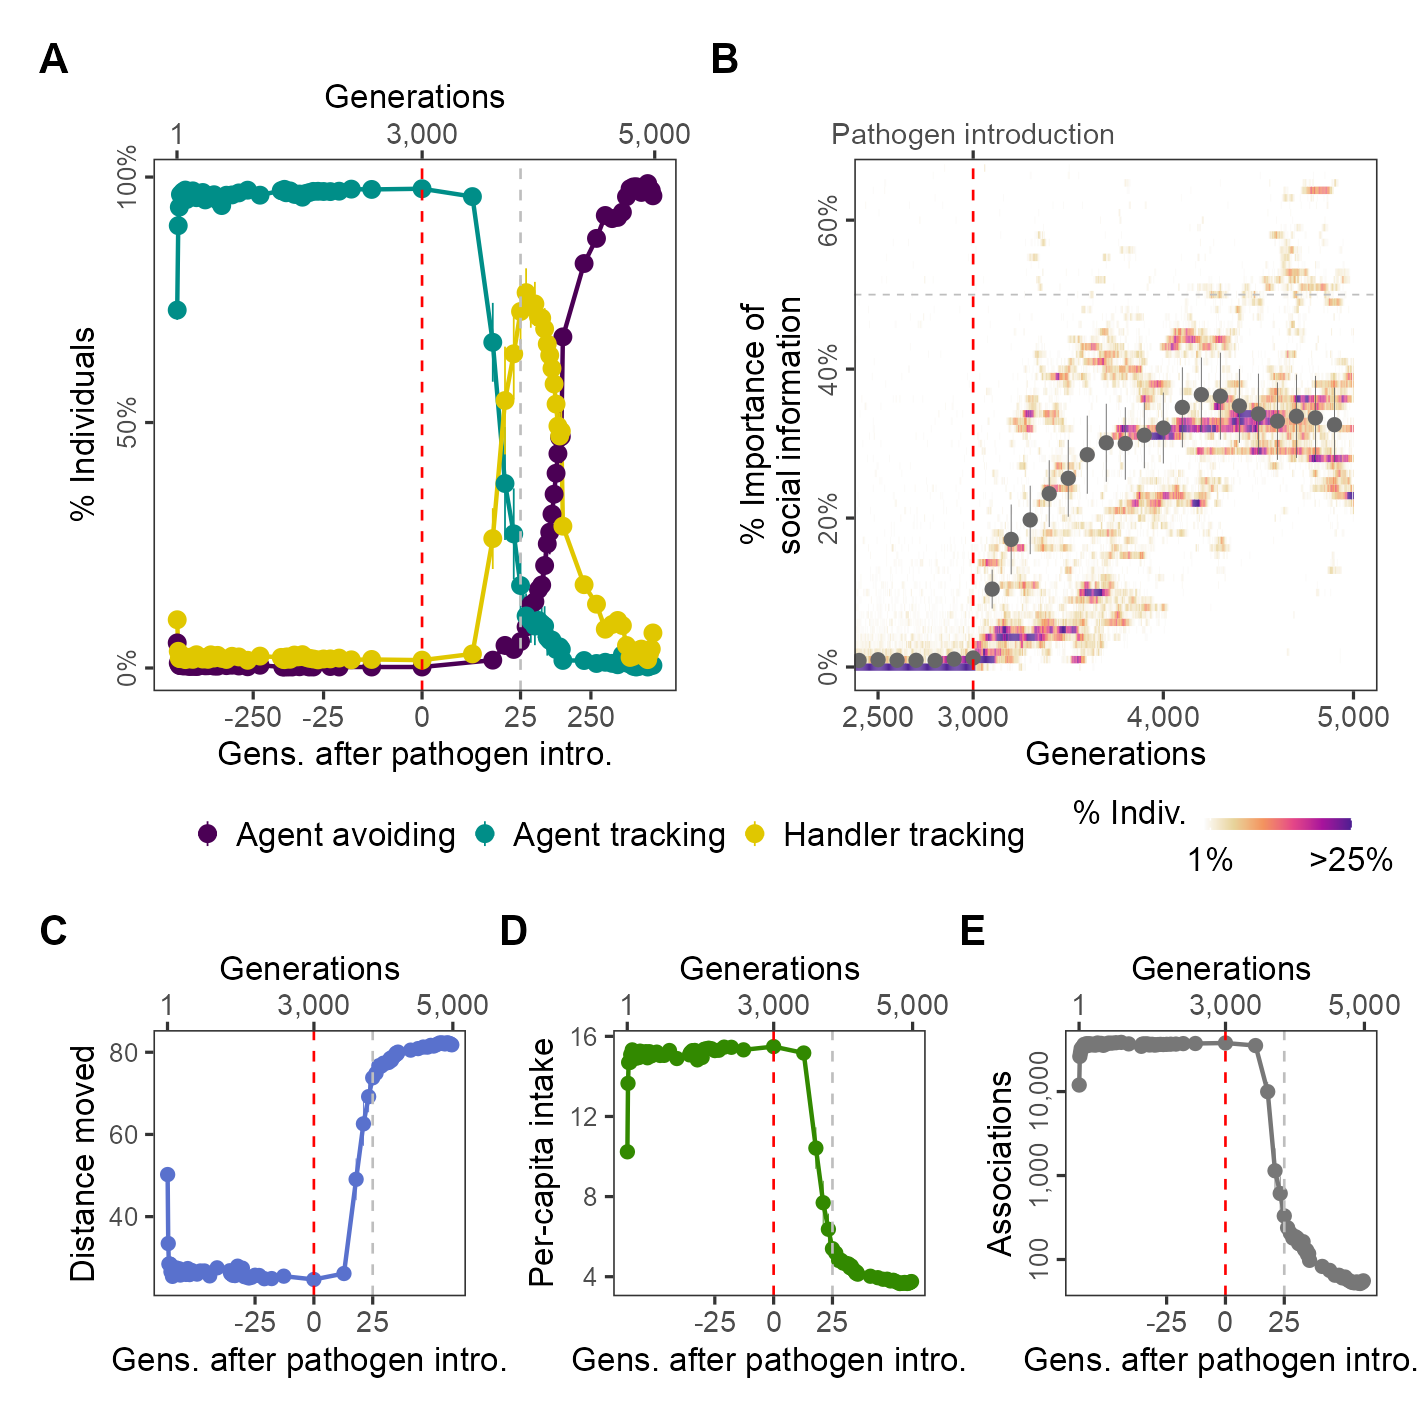
\includegraphics[width=0.9\linewidth]{figures/pathomove/fig_01.png}
    \caption{
        \textbf{Pathogen introduction leads to rapid evolutionary changes in social information use, with cascading effects on population ecological outcomes.}
        \textbf{(A)} Before pathogen introduction in the default scenario ($R$ = 2, $\delta E$ = 0.25), populations rapidly evolve a social movement strategy that tracks all other individuals (`agent tracking'; $G \leq$ 3,000) --- however, their overall movement strategy is primarily guided by the presence of food items (\textbf{(B)}).
        Pathogen introduction leads to the rapid replacement, within 25 generations, of agent tracking with `handler tracking' (preference for successful foragers; 3,000 $< G <$ 3,025), and within 250 generations, with `agent avoidance' (avoidance of both successful and unsuccessful foragers; $G >$ 3,250).
        \textbf{(B)} After pathogen introduction ($G >$ 3,000), the importance of social cues (the presence of other individuals; the sum of the absolute, normalised preferences $sH, sN$) increases substantially on average (grey points).
        Additionally, there is significant variation in the importance of social cues to individuals (shaded regions), which is not captured by the mean or standard error.
        At $G$ = 4,000, for example, social information comprises $\approx$ 30\% of most individuals' movement strategies, but has both higher ($>$ 40\%) and lower weightage ($\approx$ 20\%) for some individuals.
        The rapid change in social movement strategies following pathogen introduction is reflected in ecological outcomes.
        Individuals, which have evolved strong aversions to other foragers, \textbf{(C)} move more on average, \textbf{(D)} have a mean per-capita intake of only 25\% of the pre-pathogen average, and \textbf{(E)} reduce associations with other individuals 100-fold.
        All panels show data averaged over 10 replicates, but shaded region in panel B shows only a single replicate for clarity.
    }
    \label{patho_fig_01}
\end{figure}

\subsection*{Ecological-scale consequences of shift in movement strategies}

In our default scenario ($R$ = 2, $\delta E$ = 0.25) the ecological and behavioural consequences of the evolutionary shift in movement strategies are drastic and similarly rapid (Fig.~\ref{patho_fig_01}C -- E; see \textit{Supplementary Material Fig. 3} for other scenarios).
There is a sharp increase in mean distance moved by individuals; while pre-introduction individuals moved ~55\% of their lifetimes on average (i.e., 55 timesteps; handling for the remainder), post-introduction, individuals move for ~80\% of their lifetimes (i.e., 80 timesteps; Fig.~\ref{patho_fig_01}C).
One reason individuals move more post-introduction is that their strategy of avoiding searching foragers (or all foragers) likely leads them to mostly move away from other individuals.
Since individuals are most likely to be found on or near resource clusters, this possibly leads to movement away from productive areas of the landscape.
This idea is supported by the rapid, four-fold drop in mean per-capita intake after pathogen introduction (Fig.~\ref{patho_fig_01}D).
The near 100-fold drop in encounters between individuals after pathogen introduction (Fig.~\ref{patho_fig_01}E) also supports this idea and suggests that most encounters were likely taking place on or near resource clusters.
These reductions in intake are equivalent to those expected from halving landscape productivity (\textit{Supplementary Material Fig. 3}).
Thus our model suggests that in addition to direct disease costs ($\delta E$), pathogen introduction, by influencing the evolution of movement strategies, may also have substantial indirect ecological effects.

\subsection*{Individual differences in social movement strategies affect population-level social structure}

The relationship between movement and avoiding associations (and further, infection) is mediated by individual differences in how exactly social information is incorporated into movement strategies.
Individuals using the agent avoiding strategy move more than handler tracking ones (Fig.~\ref{patho_fig_02}A), about 85\% of their lifetime (default scenario: $R$ = 2; $\delta E$ = 0.25).
At this limit, every step moved allows them to avoid approximately 2 encounters with other individuals.
Handler tracking individuals move much less ($\sim$ 60\% -- 80\%), but are able to avoid approximately 20 encounters with other individuals with every extra step.
These differences may explain why agent avoiding and handler tracking individuals have very similar mean infection rates, at $\sim$ 25\% and $\sim$ 33\% respectively (Fig.~\ref{patho_fig_02}B).
All other strategies, including the agent tracking strategy common in pre-introduction populations, are barely able to translate increased movement into fewer associations (Fig.~\ref{patho_fig_02}A).
These strategies have a wide range of infection rates (Fig.~\ref{patho_fig_02}B), potentially because they are very rare --- these likely represent mutants that do not give rise to persistent lineages.

\begin{figure}[!h]
    \centering
    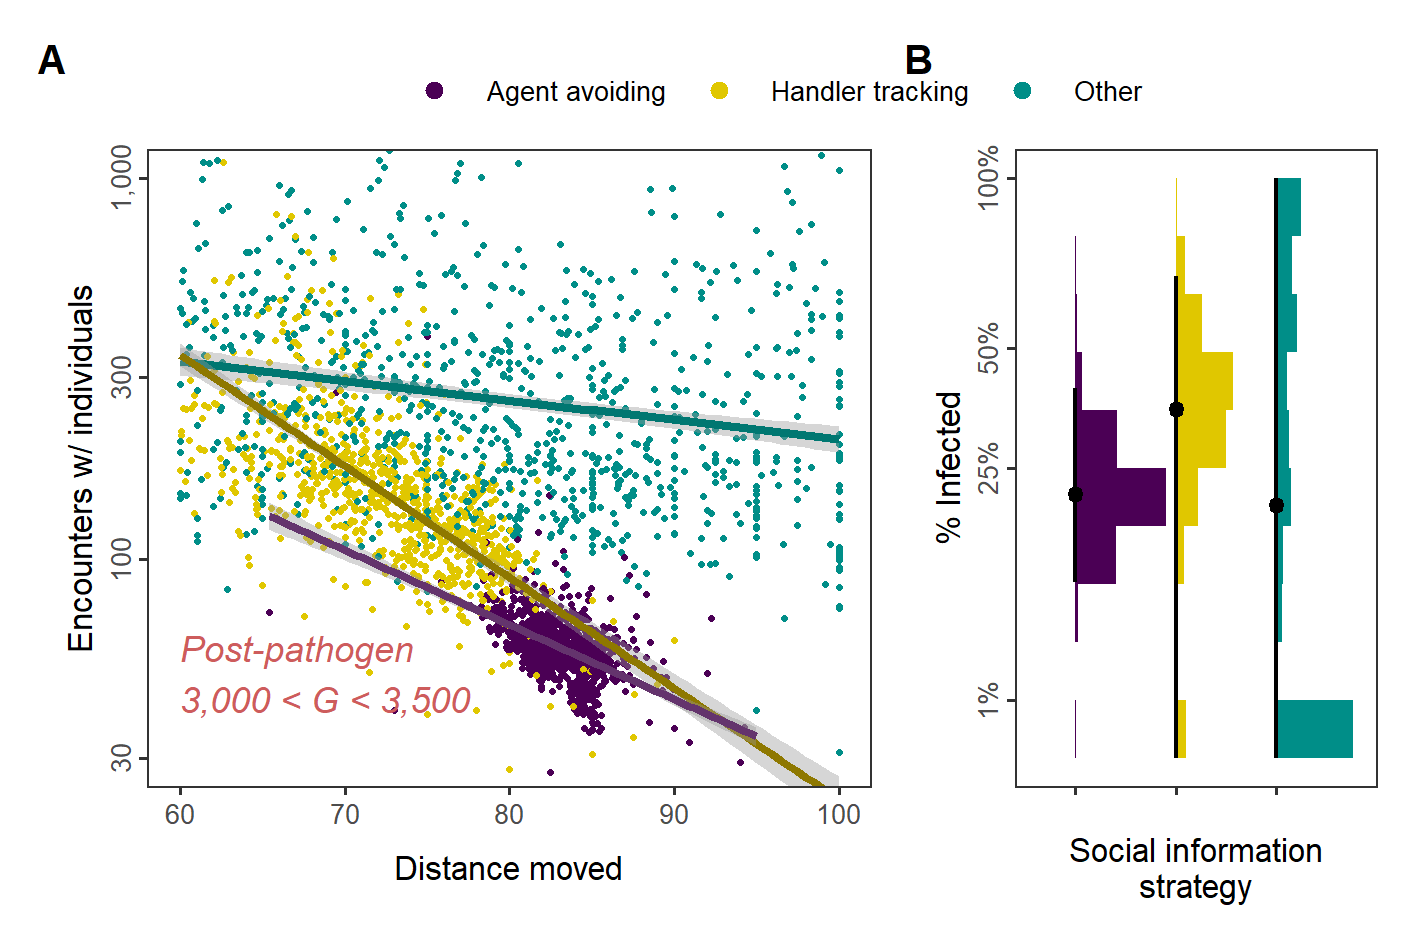
\includegraphics[width=0.9\linewidth]{figures/pathomove/fig_02.png}
    \caption{
        \textbf{Social movement strategies trade movement for associations through dynamic social distancing, leading to differences in infection rates.}
        In post-introduction populations (3,000 $<$ G $<$ 3,500), \textbf{(A)} both agent avoiding and handler tracking individuals can reduce encounters with other individuals by moving to avoid other foragers (dynamic social distancing).
        Handler tracking individuals have many more encounters than agent avoiding individuals, but surprisingly, are better able to reduce encounters through increased movement.
        Individuals using other strategies (mostly agent tracking) have a wider range of movement distances, but cannot efficiently avoid other foragers by moving more.
        \textbf{(B)} Avoiding all other foragers leads to marginally lower infection rates than tracking successful foragers (and avoiding unsuccessful ones; handler tracking).
        Surprisingly, rare pre-introduction strategies such as following any nearby individuals (agent tracking) may also have low infection rates, potentially due to their rarity.
        Panel A shows linear model fits with a log scale Y-axis; panel B shows infection rates; all data represent generation- and replicate-specific means (3,000 $< G <$ 3,500; $R$ = 2, $\delta E$ = 0.25).
    }\label{patho_fig_02}
\end{figure}

Following pathogen introduction, the mixture of individual-level movement strategies experiences a substantial re-organisation of emergent spatial and social structure at the population level (default scenario: $R$ = 2; $\delta E$ = 0.25).
Pre-introduction populations are strongly clustered in space (Fig.~\ref{patho_fig_03}A), due to movement strategies that favour following most other foragers.
This spatial proximity means that most individuals encounter each other at least once, leading to numerous unique partners (the `degree') for each forager (Fig.~\ref{patho_fig_03} inset A).
In contrast, post-introduction populations are much more dispersed across the landscape (Fig.~\ref{patho_fig_03}B), reflecting movement strategies which lead to near-perpetual movement to avoid associations; a sort of dynamic social distancing \citep{pusceddu2021}.
This dispersed population structure means that most foragers encounter fewer than 10\% of the population over their lifetime (Fig.~\ref{patho_fig_03} inset B).

\afterpage{
    \begin{sidewaysfigure}[p]
        \centering
        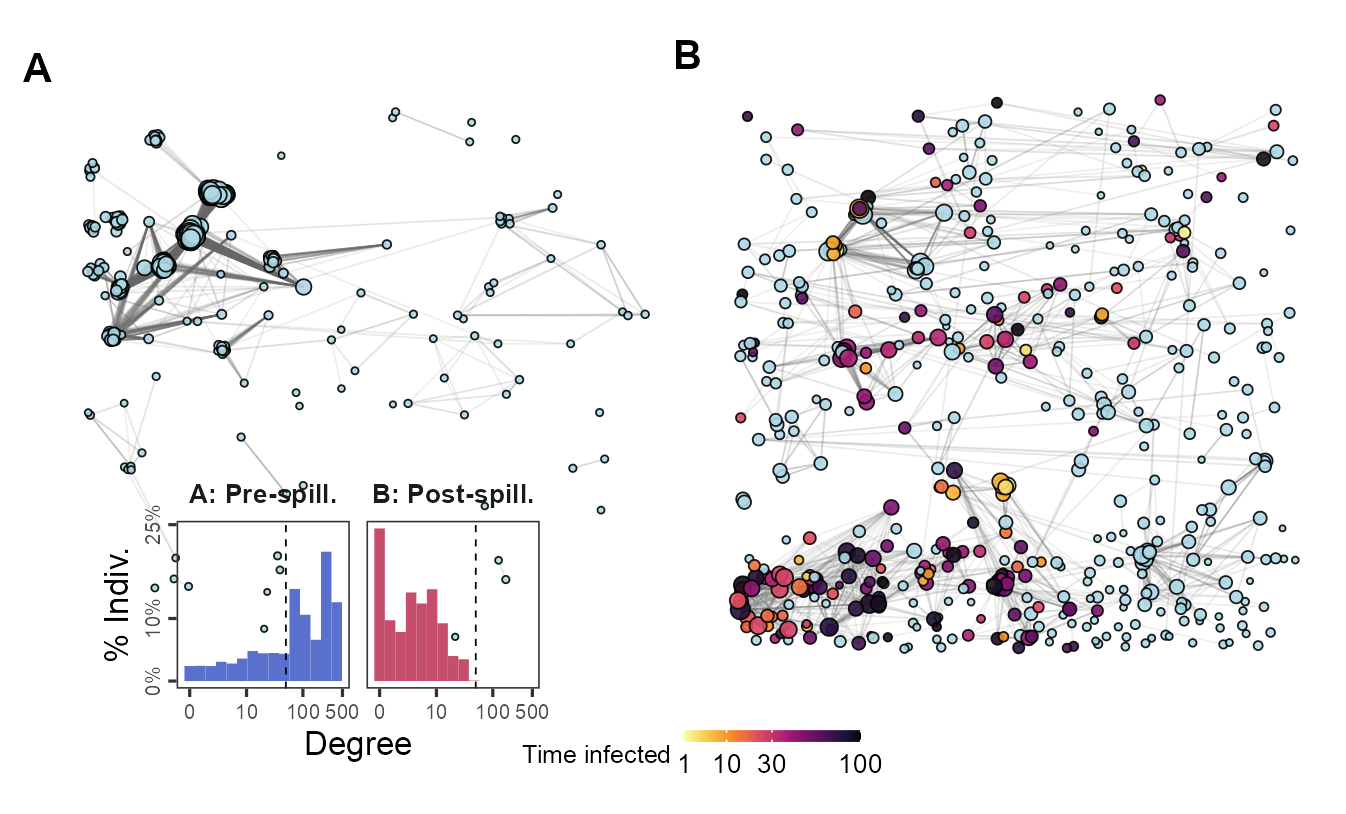
\includegraphics[width=0.7\linewidth]{figures/pathomove/fig_03.png}
        % width=8.7cm
        \caption{
            \textbf{Reduced spatial-social clustering in the presence of an infectious pathogen.}
            Pre-introduction populations (\textbf{A}; G = 3,000) are substantially more spatially clustered than post-introduction populations (\textbf{B}; $G$ = 3,500).
            This clustering means that pre-introduction individuals encounter many more unique neighbours (\textbf{inset A}) than do post-introduction individuals (\textbf{inset B}).
            Dashed grey line represents 10\% of individuals encountered (N = 50).
            The more spread-out networks in post-introduction populations suggest that most foragers move substantially from their initial locations over their lifetime, leading to associations with foragers from all over the landscape.
            Main panels show social networks from a single replicate of the default scenario ($R$ = 2, $\delta E$ = 0.25); \textbf{(A)} shows all 500 individuals, which are extremely spatially clustered.
            Nodes representing individuals, connections representing pairwise encounters, and node size representing the total number of encounters (larger circles = more encounters).
            In main panels, colours indicate how long individuals have been infected: darker colours indicate longer infection, light blue indicates no infection.
            Main panels show a single unique simulation run; inset shows degree distributions from 10 simulation replicates, and the X-axis is log-scaled.
        }\label{patho_fig_03}
    \end{sidewaysfigure}
}


\subsection*{Pathogen-adapted movement strategies make animal societies more resilient to the spread of disease}

Nearly every individual in the generations just after pathogen introduction was infected.
However, tracking the evolutionary change in movement strategies, the number of infected individuals fell to just about 50\% within 25 generations (Fig.~\ref{patho_fig_04}A).
To examine potential pathogen spread in pre-introduction populations, we ran a simple epidemiological model on the social networks emerging from individuals' movements before and after pathogen introduction (pre-introduction: $G =$ 3,000; post-introduction: $G =$ 3,500).
We modelled two diseases, \textit{(i)} first, a disease requiring one encounter,and \textit{(ii)} second, a disease requiring ten encounters between individuals for a potential transmission event (transmission rate $\beta$ = 5.0, recovery rate $\gamma$ = 1.0).
Both the single encounter and multiple encounter diseases would infect 75\% -- 80\% of individuals when spreading through the networks of pre-introduction populations (Fig.~\ref{patho_fig_04}B).
Pathogen-adapted populations' social networks are more resilient to both the single encounter and multiple encounter disease, compared to their pre-introduction, pathogen-naive ancestors (Fig.~\ref{patho_fig_04}B).
Less than 50\% of post-introduction populations were finally infected by the single encounter disease, compared with $>$ 75\% of pre-introduction, pathogen-naive ancestors.
In pathogen-adapted populations, the spread of the multiple encounter disease was even slower (ever infected: $\approx$ 20\%), as these social networks are sparser and individuals are more weakly connected (Fig.~\ref{patho_fig_04}B; see Fig.~\ref{patho_fig_03}B).

\begin{figure}[!h]
    \centering
    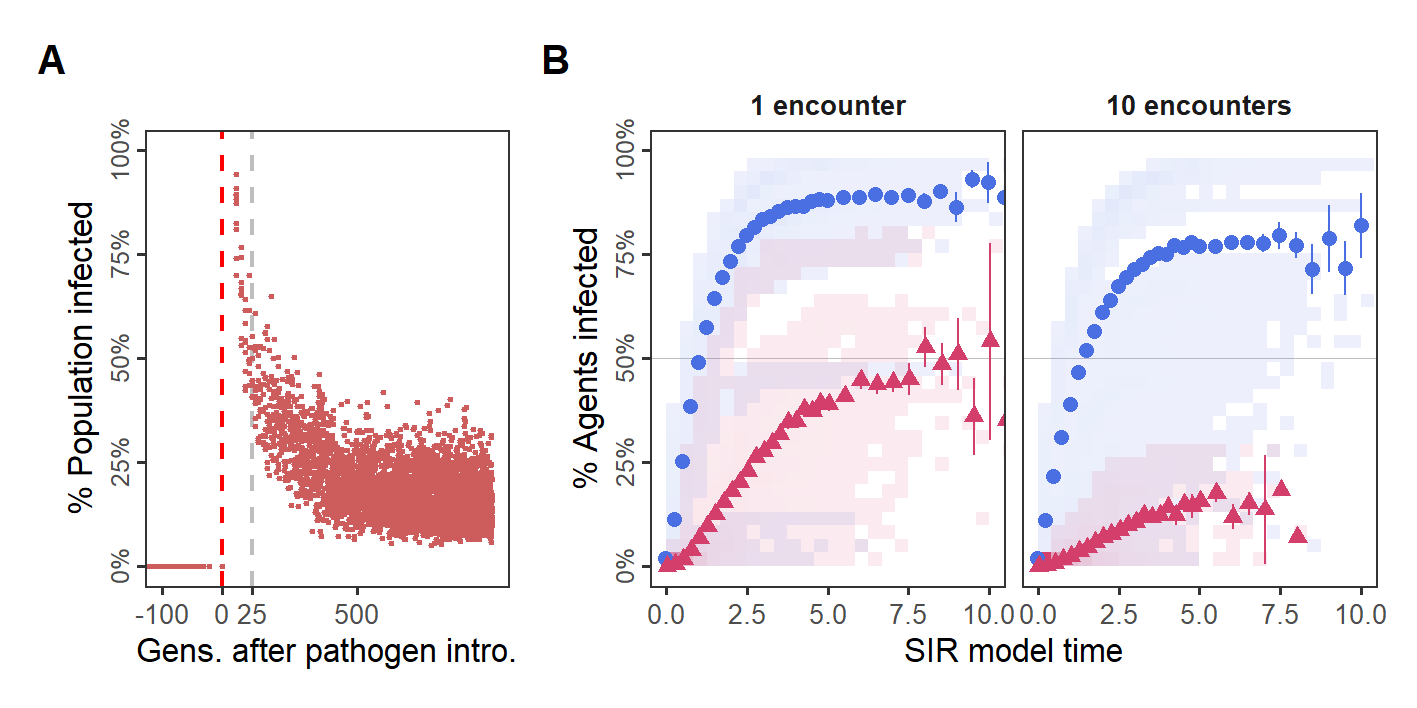
\includegraphics[width=0.9\linewidth]{figures/pathomove/fig_04.png}
    % width=8.7cm
    \caption{
        \textbf{The spread of disease is slowed in populations adapted to the presence of an infectious pathogen.}
        \textbf{(A)} In the first generations following pathogen introduction, nearly every single individual in the population is infected (default scenario: $R$ = 2, $\delta E$ = 0.25).
        However, within 25 generations, tracking the evolutionary shift towards movement strategies that avoid some or all other individuals, only about 50\% of individuals are ever infected; this drops further to a stable $\approx$ 20\% within 500 generations after pathogen introduction.
        \textbf{(B)} The progression of two hypothetical diseases (transmission rate $\beta$ = 5.0, recovery rate $\gamma$ = 1.0), requiring  a single encounter, or 10 encounters for a potential transmission.
        A simple SIR model on the emergent social networks of pre- (blue dots) and post-introduction (red triangles) populations ($G$ = 3,000, and $G$ = 3,500) shows that the transmission of both diseases is reduced in populations with disease-adapted movement strategies.
        Panels show means of 25 SIR model replicates, run on emergent social networks from each of 10 simulation replicates in the default scenario ($R$ = 2, $\delta E$ = 0.25).
    }\label{patho_fig_04}
\end{figure}

\subsection*{Landscape productivity and infection cost influence which social movement strategies evolve}

We ran our model with nine different combinations of landscape productivity ($R \in $ 1, 2, 5) and infection cost per timestep ($\delta E \in$ 0.1, 0.25, 0.5).
Initially, in the absence of the pathogen, landscape productivity alone determines the benefits of social information, and thus which social movement strategies evolve (Fig.~\ref{patho_fig_05}).
On low-productivity landscapes ($R$ = 1), social information is valuable as direct resource cues are scarce; here, the handler-tracking strategy persists.
On high-productivity landscapes ($R \in$ 2, 5), social information is less valuable as individuals can directly detect food items more often; here, the agent tracking strategy is most common.
%%
Across scenarios, the introduction of the infectious pathogen leads to a rapid evolutionary shift in social movement strategies.
The benefits of social information (mediated by landscape productivity), and infection cost jointly determine how pathogen introduction alters the mix of social movement strategies.
When the benefit of social information balances the cost of infection, the handler tracking strategy is common ($R$ = 1, $\delta E$ = 0.1; $R$ = 5, $\delta E$ = 0.25).
When social information benefits are lower than infection costs (e.g. $\delta E$ = 0.5), the agent avoiding strategy is common.
Landscape productivity can also directly balance infection costs: on high-productivity landscapes with low infection costs ($R \in$ 2, 5, $\delta E$ = 0.1), pathogen introduction does not cause a shift in movement strategies, and the agent tracking strategy remains prevalent.

\begin{figure}[!h]
    \centering
    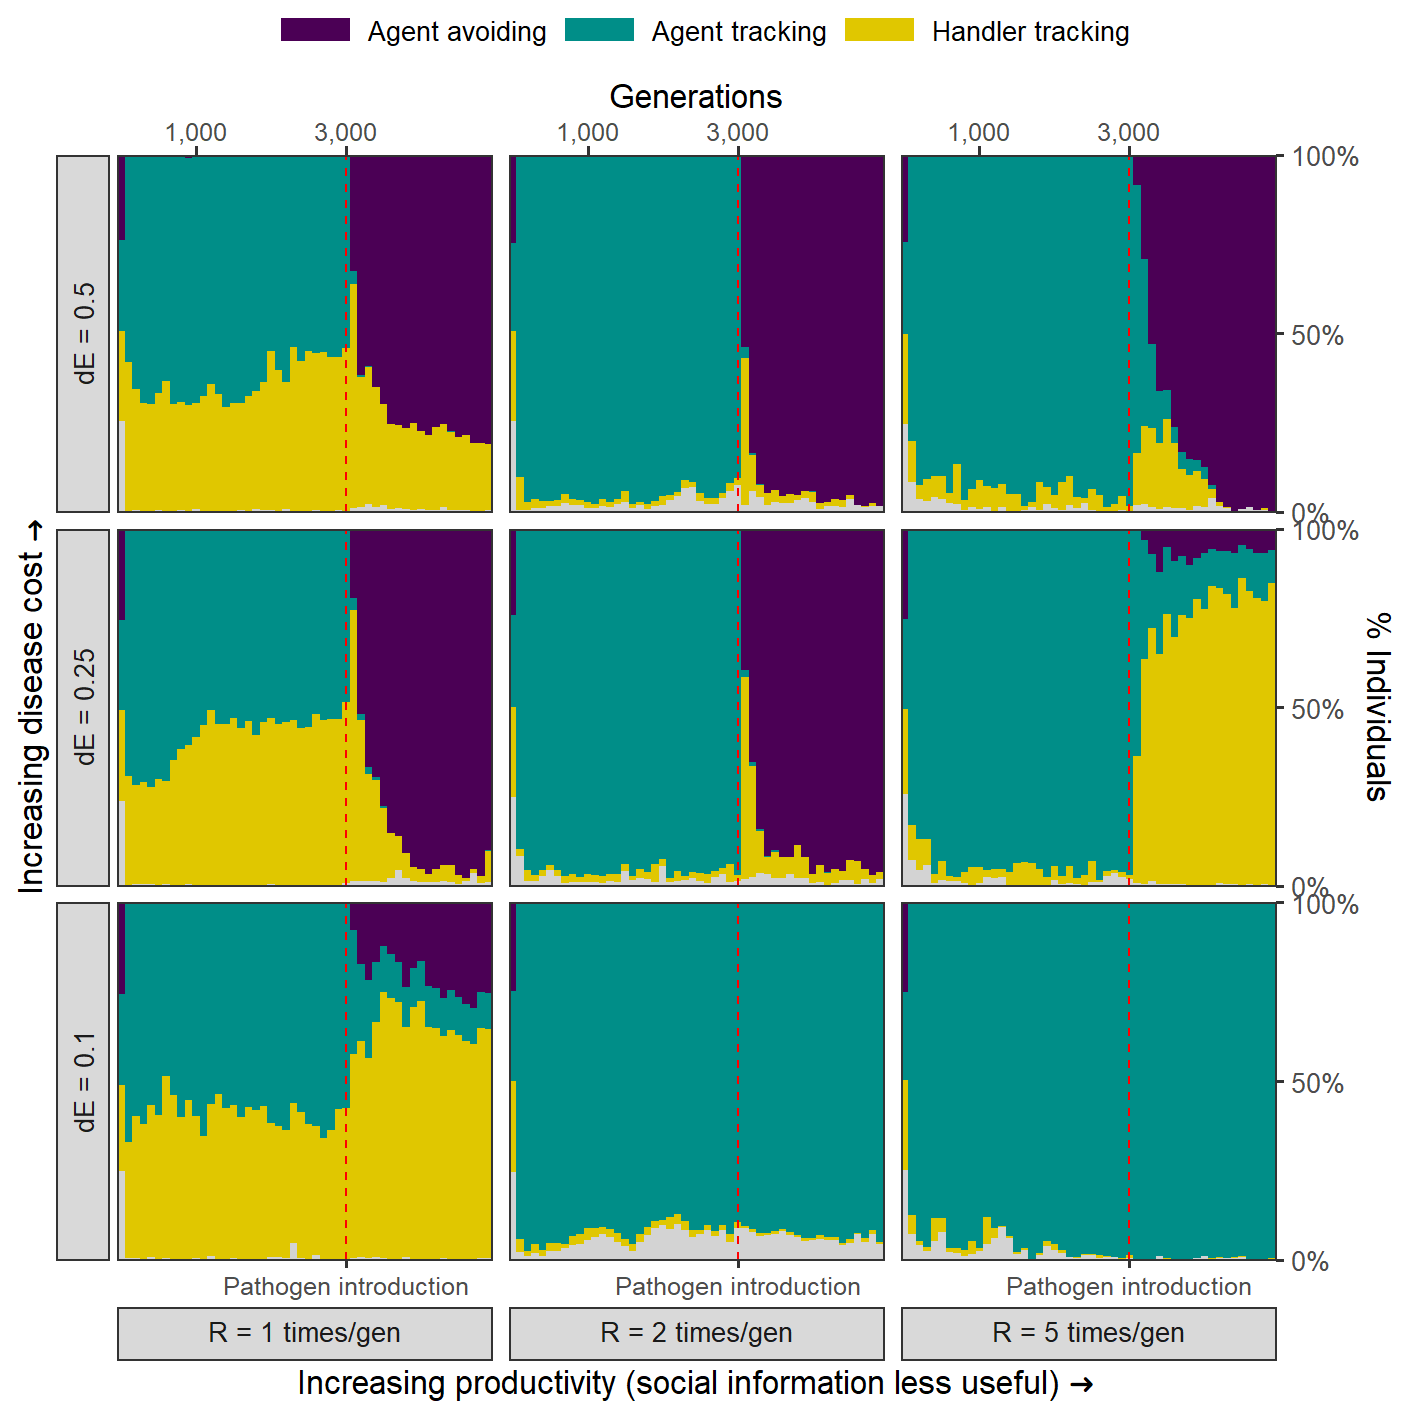
\includegraphics[width=0.9\linewidth]{figures/pathomove/fig_05.png}
    % width=8.7cm
    \caption{
        \textbf{The balance of infection cost and the usefulness of social information together shape the rapid evolutionary change in movement strategies triggered by pathogen introduction.}
        Pre-introduction ($G$ = 3,00; dashed line) populations contain a mix of individuals that either track all foragers (agent tracking), or only successful foragers (handler tracking).
        Handler tracking is more common on low-productivity landscapes ($R$ = 1), where social information is more useful to find patchily distributed resources.
        After pathogen introduction, the agent avoidance (avoiding both successful and unsuccessful foragers) emerges and rapidly becomes the most common strategy when infection costs are high ($\delta E \geq$ 0.25), and on low-productivity landscapes.
        When the benefit of social information outweighs the costs of infection, the handler tracking strategy is common.
        This occurs both when productivity is low ($R$ = 1) and infection costs are low ($\delta E$ = 0.1), but also when productivity is high ($R$ = 5) with intermediate infection costs ($\delta E$ = 0.25).
        In scenarios of high landscape productivity combined with low infection costs (e.g. $R$ = 5, $\delta E$ = 0.1), the agent tracking strategy persists beyond pathogen introduction.
        All panels show mean frequencies over 10 replicate simulations in 100 generation bins; frequencies are stacked.
        Grey areas show the relatively uncommon `non-handler' tracking strategy.
    }\label{patho_fig_05}
\end{figure}

\section*{Discussion}

Our model is among the first to demonstrate the tension inherent to sociality under the risk of an infectious pathogen, in an explicitly spatial context.
We show how populations, initially evolved to find patchily distributed food using social information, rapidly evolve to eschew social encounters when an infectious pathogen is introduced.
Our work shows how qualitatively and quantitatively different social movement strategies --- each making a different trade-off between social information and infection risk --- can co-exist in a single population.

We expected that prior to pathogen introduction, exploitation competition should promote the use of high-quality social information, and the avoidance of potential competitors \citep[handler tracking;][]{gupte2021a}.
We found that the usefulness of social information affected this outcome quite strongly, as handler tracking was most common on low-productivity landscapes ($R$ = 1), where social information is crucial to finding resources (see \textit{Model and Analysis}).
Our current model's landscape clusters are more sparsely and irregularly distributed than in our previous work \citep{gupte2021a}, and individuals are initialised near their parent's final location (see \textit{Supplementary Material Fig. 2, 4}).
This leads to `ecological inheritance' whereby successful individuals on or near resource clusters pass their favourable positions on to their offspring \citep{badyaev2009}.
Avoiding potential competitors thus correlates with avoiding profitable areas.
This leads to the persistence of the indiscriminately social agent tracking strategy, despite the evident costs of exploitation competition (see \textit{Supplementary Material Section 3.2} for an alternative implementation).
We found an unexpectedly rapid evolutionary shift, within 25 generations, in individual movement strategies following pathogen introduction.
This is much more rapid than the timescales usually associated with the evolution of complex traits such as sociality.
This change actually occurs over fewer generations than over which key aspects of animal culture and ecology, such as migration routes, are established through social learning \citep{jesmer2018,cantor2021}.
Current and expected cross-species transmissions of novel pathogens \citep{carlson2021,pusceddu2021} should thus prompt concern that the evolutionary consequences of pathogen introduction could slow the transmission of, and erode, animal culture \citep{cantor2021}.

Avoiding potentially infectious individuals is a key component of navigating the `landscape of disgust' \citep{weinstein2018}.
To navigate this landscape effectively, animals must first be sensitive, or become more sensitive, to cues of high transmission risk.
Our results show that such sensitivity can rapidly evolve following the introduction of a novel pathogen, leading to strong qualitative changes in movement strategies within 100 generations.
Furthermore, on average, individuals' sensitivity to social movement cues actually increases after pathogen introduction.
However, there was substantial between-individual variation in the importance of social cues overall, even after a specific movement strategy had become dominant.
A mix of individuals with different sensitivities to social cues, relative to resource cues, is key to the evolution of large-scale collective behaviours, such as migration \citep{guttal2010}.
Our work suggests how in the long term (about 500 generations), by leading to the necessary diversity in social movement strategies, a novel pathogen may actually lay the groundwork for the evolution of more complex collective behaviour.
The emergence of individual variation in social movement strategies, and especially the trade-off between movement, associations, and infection risk also suggests a clear mechanism by which sociality could evolve as a personality trait \citep[][]{gartland2021}.

The evolutionary changes triggered by pathogen introduction were strongly and predictably controlled by the combination of landscape productivity ($R$) and infection cost ($\delta E$).
Productivity can be seen in another context: as a proxy for the usefulness of social information.
The benefits of grouping, relative to the costs of infection, can also influence sociality in the context of disease \citep{almberg2015,ezenwa2016}.
Social information benefits in a disease context are often modelled as a single parameter, with no mechanistic relationship with the subject of the information (e.g. food, predators; see e.g. \citealt{ashby2022}). 
In contrast, social information benefits in our model are emergent outcomes of animal movement and foraging mechanisms.
Our model's predictions may help explain intra- and inter-specific diversity in social systems across contexts that differ in the usefulness of social information and disease risk \citep{lott1991, sah2018}.
At the population level, this suggests one pathway by which gregarious, clustered species, which are expected to be more at risk from transmissible pathogens \citep{sah2018}, could transition to a more solitary social organisation over evolutionary timescales.
More positively, our results show that animals may be able to adapt relatively quickly to the spillover and eventual persistence of infectious pathogens, even when they cannot specifically detect and avoid infected individuals \citep{stroeymeyt2018}.

Ecological models expect even isolated pathogen outbreaks, such as that of swine fever in wild boar, to last over a decade due to interacting effects of host movement and landscape structure \citep{scherer2020}.
These outbreaks are expected to have substantial cascading effects for landscape and community ecology \citep{monk2022}.
Our model shows that rapid, disease-dominated ecological cascades --- individuals have less intake, exerting less top-down pressure on their resource --- can occur even without mortality effects, due to evolutionary shifts in movement alone.
Furthermore, our results suggest that selection against sociality (usually held constant in ecological models) could bring infection outbreaks under control more swiftly than predicted, as the population shifts from gregarious to solitary.
Nonetheless, the altered ecological state (here, less resource consumption, as in \citealt{monk2022}) may be maintained long after --- and indeed because --- a population has adapted to be less social in the presence of a pathogen.
Our network epidemiological models suggest that the spread of pathogens and parasites that are better transmitted by actual social contact (e.g. helminths), rather than simply proximity (e.g. viruses) \citep{rimbach2015}, may be lower in pathogen-adapted populations.
On one hand, this could reduce the prevalence and disease burden of previous endemic pathogens adapted to a more social host.
On the other hand, increased dispersal over the landscape may make animals more likely to widely transmit certain pathogens to their environment, and pick up these pathogens in turn \citep[][]{rimbach2015,weinstein2018,scherer2020}.

Our infectious pathogen is easily transmitted through proximity, and causes a chronic yet non-fatal disease; though realistic, these assumptions cannot capture the full diversity of pathogens and their dynamics \citep{white2018,scherer2020, lunn2021}.
More detailed mechanistic modelling would have to account for the differential effects of proximity and actual social contacts on transmission \citep{rimbach2015}.
The most pressing epizootics are fatal, causing mass mortality in mammals \citep{blehert2009, fereidouni2019} and amphibians \citep{scheele2019,sanderson2020}.
Whether such sharp, temporally restricted outbreaks result in substantial evolutionary pressure against sociality is unclear.
Comparing sociality before and after an unexpected pathogen spillover \citep[as in][]{kuchipudi2022} is likely to be challenging, not least because data on past and ongoing host-pathogen introduction events is sparse.
Our model then is especially suited to longer-term outbreaks in which populations are repeatedly exposed to novel pathogens (or strains), such as wild boar swine fever outbreaks \citep{scherer2020}, avian influenza in Arctic migratory birds \citep{globconsorth5n82016}, or the recent introduction of Covid-19 to deer \citep{kuchipudi2022}.

Pathogens also typically have much shorter generation times than their hosts.
Analytical models expect pathogen attributes to rapidly co-evolve to match host population attributes (e.g. sociality and immune resistance) \citep[][]{bonds2005,prado2009,ashby2022}.
Such models treat pathogens --- just as they do host animals --- in relatively simple, non-mechanistic ways.
Pathogens are primarily expected to evolve to a virulence that promotes between-host transmission \citep{bonds2005}.
Our mechanistic model does not explicitly consider host-pathogen co-evolutionary dynamics, as this complexity was beyond the scope of our general, conceptual model.
Adding pathogen evolutionary dynamics to a mechanistic individual-based model would require careful consideration of \textit{(i)} the costs the pathogen imposes on its hosts, and \textit{(ii)} how it transmits between hosts, both within and between generations.
We expect that multiple pathogen strategies could coexist in a host population that itself has multiple social movement strategies.

Our mechanistic model, combining animal movement and plausible disease transmission, extends current understanding of the evolutionary consequences of individual spatial-social ecology \citep{webber2018,albery2021,webber2022}.
We generate consistent predictions of marked and swift evolutionary shifts in social movement strategies that could plausibly be tested over the timescales of some long-term animal tracking studies \citep{wilber2022}.
Our social information-based movement strategies are made up of continuous values that place individuals on a two-dimensional trait space of relative preferences (or aversions) for successful and unsuccessful foragers (see \textit{Model and Analysis}; see also \citealt{gupte2021a}).
Such social movement strategies could already be revealed for free-living animals using newer step-selection approaches \citep{avgar2016}, combined with the simultaneous, high-throughput tracking of many hundreds of animals in an area \citep{nathan2022}.
More immediately, studying the movement ecology of animals across a cline of pathogen prevalence could help test the predictions of this and similar models \citep{wilber2022}.
Given that infection patterns can change rapidly in space even in small, well-mixed populations \citep{albery2022}, the systems that could be used to test these phenomena may be widespread and easily available.
Finally, our general modelling framework, correctly parameterised to suit specific animal systems, could provide useful insights in the future to guide the long-term management of wildlife populations.

% \subsection*{Data and Code Availability}

% The \textit{Pathomove} simulation model code is available on Zenodo at https://zenodo.org/record/6331816, and on Github at github.com/pratikunterwegs/pathomove.
% A reference dataset with 10 replicates of the parameter combinations presented here is archived on Zenodo at: https://zenodo.org/record/6331757.
% Code to run the simulations and analyse the output is on Zenodo at https://zenodo.org/record/6341440, and on Github at: 
% github.com/pratikunterwegs/patho-move-evol.

% \subsection*{Acknowledgements}
% We thank Jan Kreider for helpful feedback on an early draft of the manuscript;
% and Thijs Janssen for help with the simulation model code.
% We thank the Center for Information Technology of the University of Groningen for providing access to the \textit{Peregrine} high performance computing cluster to run simulations.
% P.R.G was supported by an Adaptive Life Programme grant made possible by the Groningen Institute for Evolutionary Life Sciences (GELIFES).
% J.G. was supported by a grand from the Netherlands Organization for Scientific Research (NWO-ALW; ALWOP.668).
% F.J.W. acknowledges funding from the European Research Council (ERC Advanced Grant No. 789240).

% \newrefcontext[sorting=nyt]
% \section*{Literature Cited}
% \printbibliography[title={Literature~Cited},heading=none]
% \end{refsection}
